\documentclass[1p]{elsarticle_modified}
%\bibliographystyle{elsarticle-num}

%\usepackage[colorlinks]{hyperref}
%\usepackage{abbrmath_seonhwa} %\Abb, \Ascr, \Acal ,\Abf, \Afrak
\usepackage{amsfonts}
\usepackage{amssymb}
\usepackage{amsmath}
\usepackage{amsthm}
\usepackage{scalefnt}
\usepackage{amsbsy}
\usepackage{kotex}
\usepackage{caption}
\usepackage{subfig}
\usepackage{color}
\usepackage{graphicx}
\usepackage{xcolor} %% white, black, red, green, blue, cyan, magenta, yellow
\usepackage{float}
\usepackage{setspace}
\usepackage{hyperref}

\usepackage{tikz}
\usetikzlibrary{arrows}

\usepackage{multirow}
\usepackage{array} % fixed length table
\usepackage{hhline}

%%%%%%%%%%%%%%%%%%%%%
\makeatletter
\renewcommand*\env@matrix[1][\arraystretch]{%
	\edef\arraystretch{#1}%
	\hskip -\arraycolsep
	\let\@ifnextchar\new@ifnextchar
	\array{*\c@MaxMatrixCols c}}
\makeatother %https://tex.stackexchange.com/questions/14071/how-can-i-increase-the-line-spacing-in-a-matrix
%%%%%%%%%%%%%%%

\usepackage[normalem]{ulem}

\newcommand{\msout}[1]{\ifmmode\text{\sout{\ensuremath{#1}}}\else\sout{#1}\fi}
%SOURCE: \msout is \stkout macro in https://tex.stackexchange.com/questions/20609/strikeout-in-math-mode

\newcommand{\cancel}[1]{
	\ifmmode
	{\color{red}\msout{#1}}
	\else
	{\color{red}\sout{#1}}
	\fi
}

\newcommand{\add}[1]{
	{\color{blue}\uwave{#1}}
}

\newcommand{\replace}[2]{
	\ifmmode
	{\color{red}\msout{#1}}{\color{blue}\uwave{#2}}
	\else
	{\color{red}\sout{#1}}{\color{blue}\uwave{#2}}
	\fi
}

\newcommand{\Sol}{\mathcal{S}} %segment
\newcommand{\D}{D} %diagram
\newcommand{\A}{\mathcal{A}} %arc


%%%%%%%%%%%%%%%%%%%%%%%%%%%%%5 test

\def\sl{\operatorname{\textup{SL}}(2,\Cbb)}
\def\psl{\operatorname{\textup{PSL}}(2,\Cbb)}
\def\quan{\mkern 1mu \triangleright \mkern 1mu}

\theoremstyle{definition}
\newtheorem{thm}{Theorem}[section]
\newtheorem{prop}[thm]{Proposition}
\newtheorem{lem}[thm]{Lemma}
\newtheorem{ques}[thm]{Question}
\newtheorem{cor}[thm]{Corollary}
\newtheorem{defn}[thm]{Definition}
\newtheorem{exam}[thm]{Example}
\newtheorem{rmk}[thm]{Remark}
\newtheorem{alg}[thm]{Algorithm}

\newcommand{\I}{\sqrt{-1}}
\begin{document}

%\begin{frontmatter}
%
%\title{Boundary parabolic representations of knots up to 8 crossings}
%
%%% Group authors per affiliation:
%\author{Yunhi Cho} 
%\address{Department of Mathematics, University of Seoul, Seoul, Korea}
%\ead{yhcho@uos.ac.kr}
%
%
%\author{Seonhwa Kim} %\fnref{s_kim}}
%\address{Center for Geometry and Physics, Institute for Basic Science, Pohang, 37673, Korea}
%\ead{ryeona17@ibs.re.kr}
%
%\author{Hyuk Kim}
%\address{Department of Mathematical Sciences, Seoul National University, Seoul 08826, Korea}
%\ead{hyukkim@snu.ac.kr}
%
%\author{Seokbeom Yoon}
%\address{Department of Mathematical Sciences, Seoul National University, Seoul, 08826,  Korea}
%\ead{sbyoon15@snu.ac.kr}
%
%\begin{abstract}
%We find all boundary parabolic representation of knots up to 8 crossings.
%
%\end{abstract}
%\begin{keyword}
%    \MSC[2010] 57M25 
%\end{keyword}
%
%\end{frontmatter}

%\linenumbers
%\tableofcontents
%
\newcommand\colored[1]{\textcolor{white}{\rule[-0.35ex]{0.8em}{1.4ex}}\kern-0.8em\color{red} #1}%
%\newcommand\colored[1]{\textcolor{white}{ #1}\kern-2.17ex	\textcolor{white}{ #1}\kern-1.81ex	\textcolor{white}{ #1}\kern-2.15ex\color{red}#1	}

{\Large $\underline{12a_{0231}~(K12a_{0231})}$}

\setlength{\tabcolsep}{10pt}
\renewcommand{\arraystretch}{1.6}
\vspace{1cm}\begin{tabular}{m{100pt}>{\centering\arraybackslash}m{274pt}}
\multirow{5}{120pt}{
	\centering
	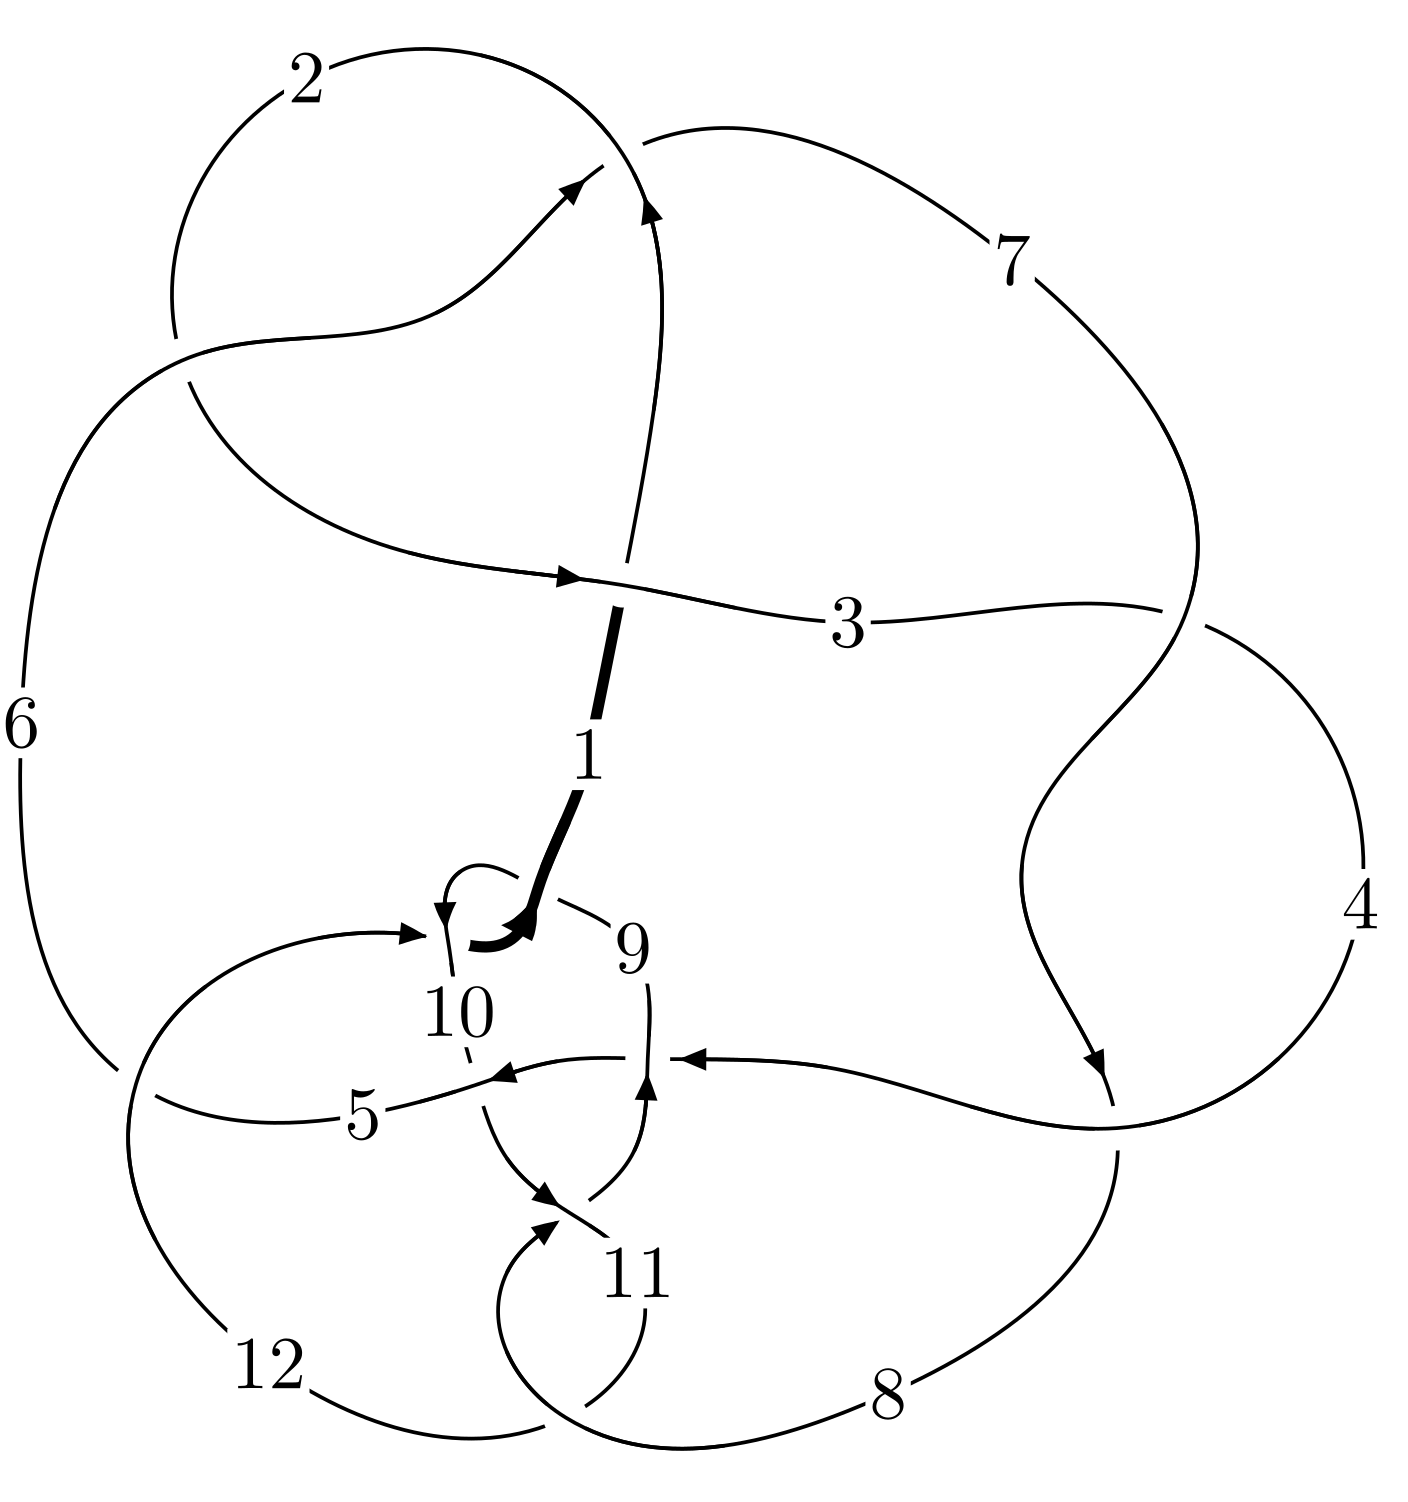
\includegraphics[width=112pt]{../../../GIT/diagram.site/Diagrams/png/1032_12a_0231.png}\\
\ \ \ A knot diagram\footnotemark}&
\allowdisplaybreaks
\textbf{Linearized knot diagam} \\
\cline{2-2}
 &
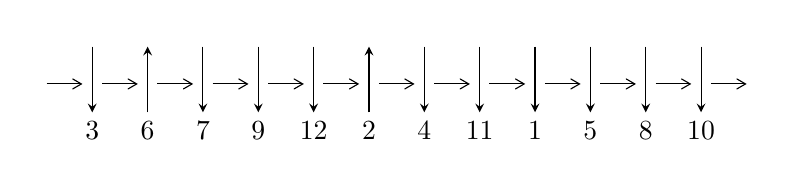
\begin{tikzpicture}[x=20pt, y=17pt]
	% nodes
	\node (C0) at (0, 0) {};
	\node (C1) at (1, 0) {};
	\node (C1U) at (1, +1) {};
	\node (C1D) at (1, -1) {3};

	\node (C2) at (2, 0) {};
	\node (C2U) at (2, +1) {};
	\node (C2D) at (2, -1) {6};

	\node (C3) at (3, 0) {};
	\node (C3U) at (3, +1) {};
	\node (C3D) at (3, -1) {7};

	\node (C4) at (4, 0) {};
	\node (C4U) at (4, +1) {};
	\node (C4D) at (4, -1) {9};

	\node (C5) at (5, 0) {};
	\node (C5U) at (5, +1) {};
	\node (C5D) at (5, -1) {12};

	\node (C6) at (6, 0) {};
	\node (C6U) at (6, +1) {};
	\node (C6D) at (6, -1) {2};

	\node (C7) at (7, 0) {};
	\node (C7U) at (7, +1) {};
	\node (C7D) at (7, -1) {4};

	\node (C8) at (8, 0) {};
	\node (C8U) at (8, +1) {};
	\node (C8D) at (8, -1) {11};

	\node (C9) at (9, 0) {};
	\node (C9U) at (9, +1) {};
	\node (C9D) at (9, -1) {1};

	\node (C10) at (10, 0) {};
	\node (C10U) at (10, +1) {};
	\node (C10D) at (10, -1) {5};

	\node (C11) at (11, 0) {};
	\node (C11U) at (11, +1) {};
	\node (C11D) at (11, -1) {8};

	\node (C12) at (12, 0) {};
	\node (C12U) at (12, +1) {};
	\node (C12D) at (12, -1) {10};
	\node (C13) at (13, 0) {};

	% arrows
	\draw[->,>={angle 60}]
	(C0) edge (C1) (C1) edge (C2) (C2) edge (C3) (C3) edge (C4) (C4) edge (C5) (C5) edge (C6) (C6) edge (C7) (C7) edge (C8) (C8) edge (C9) (C9) edge (C10) (C10) edge (C11) (C11) edge (C12) (C12) edge (C13) ;	\draw[->,>=stealth]
	(C1U) edge (C1D) (C2D) edge (C2U) (C3U) edge (C3D) (C4U) edge (C4D) (C5U) edge (C5D) (C6D) edge (C6U) (C7U) edge (C7D) (C8U) edge (C8D) (C9U) edge (C9D) (C10U) edge (C10D) (C11U) edge (C11D) (C12U) edge (C12D) ;
	\end{tikzpicture} \\
\hhline{~~} \\& 
\textbf{Solving Sequence} \\ \cline{2-2} 
 &
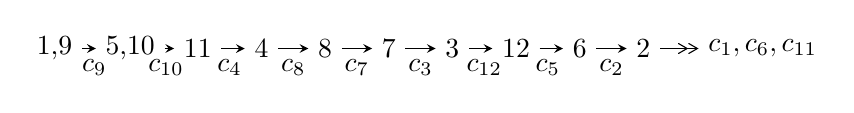
\begin{tikzpicture}[x=23pt, y=7pt]
	% node
	\node (A0) at (-1/8, 0) {1,9};
	\node (A1) at (17/16, 0) {5,10};
	\node (A2) at (17/8, 0) {11};
	\node (A3) at (25/8, 0) {4};
	\node (A4) at (33/8, 0) {8};
	\node (A5) at (41/8, 0) {7};
	\node (A6) at (49/8, 0) {3};
	\node (A7) at (57/8, 0) {12};
	\node (A8) at (65/8, 0) {6};
	\node (A9) at (73/8, 0) {2};
	\node (C1) at (1/2, -1) {$c_{9}$};
	\node (C2) at (13/8, -1) {$c_{10}$};
	\node (C3) at (21/8, -1) {$c_{4}$};
	\node (C4) at (29/8, -1) {$c_{8}$};
	\node (C5) at (37/8, -1) {$c_{7}$};
	\node (C6) at (45/8, -1) {$c_{3}$};
	\node (C7) at (53/8, -1) {$c_{12}$};
	\node (C8) at (61/8, -1) {$c_{5}$};
	\node (C9) at (69/8, -1) {$c_{2}$};
	\node (A10) at (11, 0) {$c_{1},c_{6},c_{11}$};

	% edge
	\draw[->,>=stealth]	
	(A0) edge (A1) (A1) edge (A2) (A2) edge (A3) (A3) edge (A4) (A4) edge (A5) (A5) edge (A6) (A6) edge (A7) (A7) edge (A8) (A8) edge (A9) ;
	\draw[->>,>={angle 60}]	
	(A9) edge (A10);
\end{tikzpicture} \\ 

\end{tabular} \\

\footnotetext{
The image of knot diagram is generated by the software ``\textbf{Draw programme}" developed by Andrew Bartholomew(\url{http://www.layer8.co.uk/maths/draw/index.htm\#Running-draw}), where we modified some parts for our purpose(\url{https://github.com/CATsTAILs/LinksPainter}).
}\phantom \\ \newline 
\centering \textbf{Ideals for irreducible components\footnotemark of $X_{\text{par}}$} 
 
\begin{align*}
I^u_{1}&=\langle 
6651 u^{44}+145618 u^{43}+\cdots+524288 b-466223,\\
\phantom{I^u_{1}}&\phantom{= \langle  }524233 u^{44}-2692162 u^{43}+\cdots+524288 a-643773,\;u^{45}-5 u^{44}+\cdots-4 u-1\rangle \\
I^u_{2}&=\langle 
1.55401\times10^{94} u^{69}+1.52437\times10^{95} u^{68}+\cdots+1.07854\times10^{94} b+7.18821\times10^{93},\\
\phantom{I^u_{2}}&\phantom{= \langle  }-1.16571\times10^{94} u^{69}-1.26580\times10^{95} u^{68}+\cdots+1.07854\times10^{94} a-8.60428\times10^{94},\\
\phantom{I^u_{2}}&\phantom{= \langle  }u^{70}+11 u^{69}+\cdots+16 u+1\rangle \\
I^u_{3}&=\langle 
b- a,\;32 a^5-16 a^4-16 a^3+4 a^2+2 a+1,\;u-1\rangle \\
I^u_{4}&=\langle 
a u+b+a- u+1,\;a^2-2 a u- a+u,\;u^2+1\rangle \\
\\
\end{align*}
\raggedright * 4 irreducible components of $\dim_{\mathbb{C}}=0$, with total 124 representations.\\
\footnotetext{All coefficients of polynomials are rational numbers. But the coefficients are sometimes approximated in decimal forms when there is not enough margin.}
\newpage
\renewcommand{\arraystretch}{1}
\centering \section*{I. $I^u_{1}= \langle 6651 u^{44}+145618 u^{43}+\cdots+524288 b-466223,\;5.24\times10^{5} u^{44}-2.69\times10^{6} u^{43}+\cdots+5.24\times10^{5} a-6.44\times10^{5},\;u^{45}-5 u^{44}+\cdots-4 u-1 \rangle$}
\flushleft \textbf{(i) Arc colorings}\\
\begin{tabular}{m{7pt} m{180pt} m{7pt} m{180pt} }
\flushright $a_{1}=$&$\begin{pmatrix}0\\u\end{pmatrix}$ \\
\flushright $a_{9}=$&$\begin{pmatrix}1\\0\end{pmatrix}$ \\
\flushright $a_{5}=$&$\begin{pmatrix}-0.999895 u^{44}+5.13489 u^{43}+\cdots+14.6410 u+1.22790\\-0.0126858 u^{44}-0.277744 u^{43}+\cdots+3.08293 u+0.889250\end{pmatrix}$ \\
\flushright $a_{10}=$&$\begin{pmatrix}1\\u^2\end{pmatrix}$ \\
\flushright $a_{11}=$&$\begin{pmatrix}\frac{1}{16} u^{44}-\frac{5}{16} u^{43}+\cdots-\frac{1}{4} u^2+\frac{31}{16} u\\u\end{pmatrix}$ \\
\flushright $a_{4}=$&$\begin{pmatrix}-1.01258 u^{44}+4.85715 u^{43}+\cdots+17.7239 u+2.11715\\-0.0126858 u^{44}-0.277744 u^{43}+\cdots+3.08293 u+0.889250\end{pmatrix}$ \\
\flushright $a_{8}=$&$\begin{pmatrix}\frac{1}{16} u^{43}-\frac{5}{16} u^{42}+\cdots-\frac{1}{4} u+\frac{15}{16}\\- u^2\end{pmatrix}$ \\
\flushright $a_{7}=$&$\begin{pmatrix}9.53674\times10^{-7} u^{44}-5.72205\times10^{-6} u^{43}+\cdots-5.00000 u+2.00000\\4.76837\times10^{-7} u^{44}-2.86102\times10^{-6} u^{43}+\cdots-1.00000 u-4.76837\times10^{-7}\end{pmatrix}$ \\
\flushright $a_{3}=$&$\begin{pmatrix}0.132458 u^{44}-0.552269 u^{43}+\cdots+10.2747 u+0.660954\\-0.193096 u^{44}+1.22194 u^{43}+\cdots+1.49102 u+0.299046\end{pmatrix}$ \\
\flushright $a_{12}=$&$\begin{pmatrix}u\\u^3+u\end{pmatrix}$ \\
\flushright $a_{6}=$&$\begin{pmatrix}-0.658722 u^{44}+3.16490 u^{43}+\cdots+13.8025 u+1.24059\\0.332701 u^{44}-1.98454 u^{43}+\cdots+1.52910 u+0.637812\end{pmatrix}$ \\
\flushright $a_{2}=$&$\begin{pmatrix}-0.0177879 u^{44}+0.166283 u^{43}+\cdots+9.80950 u-1.04152\\-0.00756836 u^{44}+0.106544 u^{43}+\cdots+1.77556 u-0.0534439\end{pmatrix}$\\&\end{tabular}
\flushleft \textbf{(ii) Obstruction class $= -1$}\\~\\
\flushleft \textbf{(iii) Cusp Shapes $= -\frac{853951}{4194304} u^{44}+\frac{1865277}{2097152} u^{43}+\cdots+\frac{22965053}{4194304} u-\frac{24110657}{4194304}$}\\~\\
\newpage\renewcommand{\arraystretch}{1}
\flushleft \textbf{(iv) u-Polynomials at the component}\newline \\
\begin{tabular}{m{50pt}|m{274pt}}
Crossings & \hspace{64pt}u-Polynomials at each crossing \\
\hline $$\begin{aligned}c_{1}\end{aligned}$$&$\begin{aligned}
&u^{45}+24 u^{44}+\cdots+145 u-16
\end{aligned}$\\
\hline $$\begin{aligned}c_{2},c_{6}\end{aligned}$$&$\begin{aligned}
&u^{45}-2 u^{44}+\cdots+5 u+4
\end{aligned}$\\
\hline $$\begin{aligned}c_{3},c_{7}\end{aligned}$$&$\begin{aligned}
&u^{45}+2 u^{44}+\cdots+621 u+292
\end{aligned}$\\
\hline $$\begin{aligned}c_{4},c_{5}\end{aligned}$$&$\begin{aligned}
&32(32 u^{45}-16 u^{44}+\cdots+12 u+4)
\end{aligned}$\\
\hline $$\begin{aligned}c_{8},c_{9},c_{11}\\c_{12}\end{aligned}$$&$\begin{aligned}
&u^{45}+5 u^{44}+\cdots-4 u+1
\end{aligned}$\\
\hline $$\begin{aligned}c_{10}\end{aligned}$$&$\begin{aligned}
&u^{45}+3 u^{44}+\cdots+5632 u+2048
\end{aligned}$\\
\hline
\end{tabular}\\~\\
\newpage\renewcommand{\arraystretch}{1}
\flushleft \textbf{(v) Riley Polynomials at the component}\newline \\
\begin{tabular}{m{50pt}|m{274pt}}
Crossings & \hspace{64pt}Riley Polynomials at each crossing \\
\hline $$\begin{aligned}c_{1}\end{aligned}$$&$\begin{aligned}
&y^{45}-4 y^{44}+\cdots+44993 y-256
\end{aligned}$\\
\hline $$\begin{aligned}c_{2},c_{6}\end{aligned}$$&$\begin{aligned}
&y^{45}+24 y^{44}+\cdots+145 y-16
\end{aligned}$\\
\hline $$\begin{aligned}c_{3},c_{7}\end{aligned}$$&$\begin{aligned}
&y^{45}-32 y^{44}+\cdots+1265729 y-85264
\end{aligned}$\\
\hline $$\begin{aligned}c_{4},c_{5}\end{aligned}$$&$\begin{aligned}
&1024(1024 y^{45}-5376 y^{44}+\cdots+320 y-16)
\end{aligned}$\\
\hline $$\begin{aligned}c_{8},c_{9},c_{11}\\c_{12}\end{aligned}$$&$\begin{aligned}
&y^{45}+17 y^{44}+\cdots-1030 y^2-1
\end{aligned}$\\
\hline $$\begin{aligned}c_{10}\end{aligned}$$&$\begin{aligned}
&y^{45}+9 y^{44}+\cdots-83623936 y-4194304
\end{aligned}$\\
\hline
\end{tabular}\\~\\
\newpage\flushleft \textbf{(vi) Complex Volumes and Cusp Shapes}
$$\begin{array}{c|c|c}  
\text{Solutions to }I^u_{1}& \I (\text{vol} + \sqrt{-1}CS) & \text{Cusp shape}\\
 \hline 
\begin{aligned}
u &= \phantom{-}0.520727 + 0.939578 I \\
a &= \phantom{-}0.758964 + 0.066469 I \\
b &= \phantom{-}0.779771 + 0.243421 I\end{aligned}
 & -4.56636 - 1.73156 I & -11.99281 + 3.31846 I \\ \hline\begin{aligned}
u &= \phantom{-}0.520727 - 0.939578 I \\
a &= \phantom{-}0.758964 - 0.066469 I \\
b &= \phantom{-}0.779771 - 0.243421 I\end{aligned}
 & -4.56636 + 1.73156 I & -11.99281 - 3.31846 I \\ \hline\begin{aligned}
u &= \phantom{-}0.420339 + 0.991396 I \\
a &= -0.974005 - 0.017820 I \\
b &= -0.710296 - 0.326186 I\end{aligned}
 & -0.21603 - 5.35749 I & -6.20050 + 6.92376 I \\ \hline\begin{aligned}
u &= \phantom{-}0.420339 - 0.991396 I \\
a &= -0.974005 + 0.017820 I \\
b &= -0.710296 + 0.326186 I\end{aligned}
 & -0.21603 + 5.35749 I & -6.20050 - 6.92376 I \\ \hline\begin{aligned}
u &= \phantom{-}0.776889 + 0.479998 I \\
a &= -0.168820 - 0.167222 I \\
b &= -0.630907 + 0.111072 I\end{aligned}
 & -2.93036 - 1.75870 I & -17.4213 + 1.7562 I \\ \hline\begin{aligned}
u &= \phantom{-}0.776889 - 0.479998 I \\
a &= -0.168820 + 0.167222 I \\
b &= -0.630907 - 0.111072 I\end{aligned}
 & -2.93036 + 1.75870 I & -17.4213 - 1.7562 I \\ \hline\begin{aligned}
u &= \phantom{-}0.217946 + 0.864786 I \\
a &= -1.40293 - 0.70903 I \\
b &= -0.536590 - 0.217455 I\end{aligned}
 & \phantom{-}2.55612 - 3.52730 I & -8.10907 + 10.18535 I \\ \hline\begin{aligned}
u &= \phantom{-}0.217946 - 0.864786 I \\
a &= -1.40293 + 0.70903 I \\
b &= -0.536590 + 0.217455 I\end{aligned}
 & \phantom{-}2.55612 + 3.52730 I & -8.10907 - 10.18535 I \\ \hline\begin{aligned}
u &= \phantom{-}0.442791 + 1.050870 I \\
a &= \phantom{-}0.933478 - 0.112856 I \\
b &= \phantom{-}0.753141 + 0.378689 I\end{aligned}
 & -3.07301 - 10.38100 I & -8.00000 + 9.73173 I \\ \hline\begin{aligned}
u &= \phantom{-}0.442791 - 1.050870 I \\
a &= \phantom{-}0.933478 + 0.112856 I \\
b &= \phantom{-}0.753141 - 0.378689 I\end{aligned}
 & -3.07301 + 10.38100 I & -8.00000 - 9.73173 I\\
 \hline 
 \end{array}$$\newpage$$\begin{array}{c|c|c}  
\text{Solutions to }I^u_{1}& \I (\text{vol} + \sqrt{-1}CS) & \text{Cusp shape}\\
 \hline 
\begin{aligned}
u &= -0.297785 + 1.113910 I \\
a &= \phantom{-}0.03350 + 2.19997 I \\
b &= \phantom{-}0.673195 - 0.752405 I\end{aligned}
 & \phantom{-}4.65659 - 0.00210 I & -3.78722 - 3.26916 I \\ \hline\begin{aligned}
u &= -0.297785 - 1.113910 I \\
a &= \phantom{-}0.03350 - 2.19997 I \\
b &= \phantom{-}0.673195 + 0.752405 I\end{aligned}
 & \phantom{-}4.65659 + 0.00210 I & -3.78722 + 3.26916 I \\ \hline\begin{aligned}
u &= \phantom{-}0.113962 + 0.805614 I \\
a &= \phantom{-}1.38924 + 1.35506 I \\
b &= \phantom{-}0.518517 + 0.141686 I\end{aligned}
 & \phantom{-}2.17122 + 1.50395 I & -11.94091 + 1.99102 I \\ \hline\begin{aligned}
u &= \phantom{-}0.113962 - 0.805614 I \\
a &= \phantom{-}1.38924 - 1.35506 I \\
b &= \phantom{-}0.518517 - 0.141686 I\end{aligned}
 & \phantom{-}2.17122 - 1.50395 I & -11.94091 - 1.99102 I \\ \hline\begin{aligned}
u &= -0.412048 + 0.695424 I \\
a &= -0.61411 - 2.35550 I \\
b &= -1.116650 - 0.046522 I\end{aligned}
 & -6.28912 + 6.14694 I & -10.86325 - 8.13273 I \\ \hline\begin{aligned}
u &= -0.412048 - 0.695424 I \\
a &= -0.61411 + 2.35550 I \\
b &= -1.116650 + 0.046522 I\end{aligned}
 & -6.28912 - 6.14694 I & -10.86325 + 8.13273 I \\ \hline\begin{aligned}
u &= \phantom{-}1.198270 + 0.098629 I \\
a &= -0.0225006 + 0.0343167 I \\
b &= -0.159457 + 0.519154 I\end{aligned}
 & -1.73909 + 1.72292 I & \phantom{-}5.26680 - 11.72526 I \\ \hline\begin{aligned}
u &= \phantom{-}1.198270 - 0.098629 I \\
a &= -0.0225006 - 0.0343167 I \\
b &= -0.159457 - 0.519154 I\end{aligned}
 & -1.73909 - 1.72292 I & \phantom{-}5.26680 + 11.72526 I \\ \hline\begin{aligned}
u &= -0.354317 + 1.160890 I \\
a &= -0.08135 - 2.03091 I \\
b &= -0.760215 + 0.900488 I\end{aligned}
 & \phantom{-}6.42066 + 5.09294 I & \phantom{-0.000000 } 0. - 6.60661 I \\ \hline\begin{aligned}
u &= -0.354317 - 1.160890 I \\
a &= -0.08135 + 2.03091 I \\
b &= -0.760215 - 0.900488 I\end{aligned}
 & \phantom{-}6.42066 - 5.09294 I & \phantom{-0.000000 -}0. + 6.60661 I\\
 \hline 
 \end{array}$$\newpage$$\begin{array}{c|c|c}  
\text{Solutions to }I^u_{1}& \I (\text{vol} + \sqrt{-1}CS) & \text{Cusp shape}\\
 \hline 
\begin{aligned}
u &= -0.470835 + 1.120420 I \\
a &= \phantom{-}0.30475 + 1.97067 I \\
b &= \phantom{-}1.051690 - 0.899049 I\end{aligned}
 & \phantom{-}1.14313 + 7.15516 I & -8.00000 - 7.04629 I \\ \hline\begin{aligned}
u &= -0.470835 - 1.120420 I \\
a &= \phantom{-}0.30475 - 1.97067 I \\
b &= \phantom{-}1.051690 + 0.899049 I\end{aligned}
 & \phantom{-}1.14313 - 7.15516 I & -8.00000 + 7.04629 I \\ \hline\begin{aligned}
u &= -0.334613 + 0.649816 I \\
a &= \phantom{-}0.57160 + 2.36102 I \\
b &= \phantom{-}0.967229 + 0.125022 I\end{aligned}
 & -2.56741 + 1.44381 I & -7.78555 - 4.48019 I \\ \hline\begin{aligned}
u &= -0.334613 - 0.649816 I \\
a &= \phantom{-}0.57160 - 2.36102 I \\
b &= \phantom{-}0.967229 - 0.125022 I\end{aligned}
 & -2.56741 - 1.44381 I & -7.78555 + 4.48019 I \\ \hline\begin{aligned}
u &= \phantom{-}1.224740 + 0.401588 I \\
a &= -0.1045230 + 0.0475191 I \\
b &= -0.584434 + 0.569316 I\end{aligned}
 & -4.17784 + 0.91994 I & \phantom{-0.000000 } 0 \\ \hline\begin{aligned}
u &= \phantom{-}1.224740 - 0.401588 I \\
a &= -0.1045230 - 0.0475191 I \\
b &= -0.584434 - 0.569316 I\end{aligned}
 & -4.17784 - 0.91994 I & \phantom{-0.000000 } 0 \\ \hline\begin{aligned}
u &= \phantom{-}1.217570 + 0.485388 I \\
a &= \phantom{-}0.1307500 - 0.0531710 I \\
b &= \phantom{-}0.691032 - 0.549753 I\end{aligned}
 & -7.82065 - 3.25322 I & \phantom{-0.000000 } 0 \\ \hline\begin{aligned}
u &= \phantom{-}1.217570 - 0.485388 I \\
a &= \phantom{-}0.1307500 + 0.0531710 I \\
b &= \phantom{-}0.691032 + 0.549753 I\end{aligned}
 & -7.82065 + 3.25322 I & \phantom{-0.000000 } 0 \\ \hline\begin{aligned}
u &= -0.375360 + 0.563080 I \\
a &= -0.54767 - 2.43496 I \\
b &= -1.010960 - 0.292068 I\end{aligned}
 & -6.31075 - 3.17495 I & -10.44526 - 1.01574 I \\ \hline\begin{aligned}
u &= -0.375360 - 0.563080 I \\
a &= -0.54767 + 2.43496 I \\
b &= -1.010960 + 0.292068 I\end{aligned}
 & -6.31075 + 3.17495 I & -10.44526 + 1.01574 I\\
 \hline 
 \end{array}$$\newpage$$\begin{array}{c|c|c}  
\text{Solutions to }I^u_{1}& \I (\text{vol} + \sqrt{-1}CS) & \text{Cusp shape}\\
 \hline 
\begin{aligned}
u &= -0.445965 + 1.253320 I \\
a &= -0.15883 - 1.79924 I \\
b &= -0.89148 + 1.18060 I\end{aligned}
 & \phantom{-}7.27138 + 7.55038 I & \phantom{-0.000000 } 0 \\ \hline\begin{aligned}
u &= -0.445965 - 1.253320 I \\
a &= -0.15883 + 1.79924 I \\
b &= -0.89148 - 1.18060 I\end{aligned}
 & \phantom{-}7.27138 - 7.55038 I & \phantom{-0.000000 } 0 \\ \hline\begin{aligned}
u &= \phantom{-}1.294890 + 0.408163 I \\
a &= \phantom{-}0.1009240 - 0.0680235 I \\
b &= \phantom{-}0.600371 - 0.662127 I\end{aligned}
 & -7.44445 + 5.45779 I & \phantom{-0.000000 } 0 \\ \hline\begin{aligned}
u &= \phantom{-}1.294890 - 0.408163 I \\
a &= \phantom{-}0.1009240 + 0.0680235 I \\
b &= \phantom{-}0.600371 + 0.662127 I\end{aligned}
 & -7.44445 - 5.45779 I & \phantom{-0.000000 } 0 \\ \hline\begin{aligned}
u &= -0.492198 + 1.284080 I \\
a &= \phantom{-}0.20751 + 1.72707 I \\
b &= \phantom{-}0.97106 - 1.28854 I\end{aligned}
 & \phantom{-}6.42111 + 12.47940 I & \phantom{-0.000000 } 0 \\ \hline\begin{aligned}
u &= -0.492198 - 1.284080 I \\
a &= \phantom{-}0.20751 - 1.72707 I \\
b &= \phantom{-}0.97106 + 1.28854 I\end{aligned}
 & \phantom{-}6.42111 - 12.47940 I & \phantom{-0.000000 } 0 \\ \hline\begin{aligned}
u &= -0.615203 + 1.260530 I \\
a &= -0.37637 - 1.68251 I \\
b &= -1.27509 + 1.33680 I\end{aligned}
 & -2.09321 + 9.43737 I & \phantom{-0.000000 } 0 \\ \hline\begin{aligned}
u &= -0.615203 - 1.260530 I \\
a &= -0.37637 + 1.68251 I \\
b &= -1.27509 - 1.33680 I\end{aligned}
 & -2.09321 - 9.43737 I & \phantom{-0.000000 } 0 \\ \hline\begin{aligned}
u &= -0.60014 + 1.29188 I \\
a &= \phantom{-}0.33986 + 1.65539 I \\
b &= \phantom{-}1.21338 - 1.39737 I\end{aligned}
 & \phantom{-}2.26103 + 13.52680 I & \phantom{-0.000000 } 0 \\ \hline\begin{aligned}
u &= -0.60014 - 1.29188 I \\
a &= \phantom{-}0.33986 - 1.65539 I \\
b &= \phantom{-}1.21338 + 1.39737 I\end{aligned}
 & \phantom{-}2.26103 - 13.52680 I & \phantom{-0.000000 } 0\\
 \hline 
 \end{array}$$\newpage$$\begin{array}{c|c|c}  
\text{Solutions to }I^u_{1}& \I (\text{vol} + \sqrt{-1}CS) & \text{Cusp shape}\\
 \hline 
\begin{aligned}
u &= -0.61764 + 1.30754 I \\
a &= -0.35102 - 1.62737 I \\
b &= -1.24080 + 1.44894 I\end{aligned}
 & -0.8748 + 18.5817 I & \phantom{-0.000000 } 0 \\ \hline\begin{aligned}
u &= -0.61764 - 1.30754 I \\
a &= -0.35102 + 1.62737 I \\
b &= -1.24080 - 1.44894 I\end{aligned}
 & -0.8748 - 18.5817 I & \phantom{-0.000000 } 0 \\ \hline\begin{aligned}
u &= \phantom{-}0.440279\phantom{ +0.000000I} \\
a &= -0.481278\phantom{ +0.000000I} \\
b &= \phantom{-}0.451961\phantom{ +0.000000I}\end{aligned}
 & -0.780322\phantom{ +0.000000I} & -12.5880\phantom{ +0.000000I} \\ \hline\begin{aligned}
u &= -0.132173 + 0.113061 I \\
a &= -0.47781 + 3.06580 I \\
b &= \phantom{-}0.221516 + 0.422164 I\end{aligned}
 & -0.50223 - 1.35791 I & -4.98318 + 4.28434 I \\ \hline\begin{aligned}
u &= -0.132173 - 0.113061 I \\
a &= -0.47781 - 3.06580 I \\
b &= \phantom{-}0.221516 - 0.422164 I\end{aligned}
 & -0.50223 + 1.35791 I & -4.98318 - 4.28434 I\\
 \hline 
 \end{array}$$\newpage\newpage\renewcommand{\arraystretch}{1}
\centering \section*{II. $I^u_{2}= \langle 1.55\times10^{94} u^{69}+1.52\times10^{95} u^{68}+\cdots+1.08\times10^{94} b+7.19\times10^{93},\;-1.17\times10^{94} u^{69}-1.27\times10^{95} u^{68}+\cdots+1.08\times10^{94} a-8.60\times10^{94},\;u^{70}+11 u^{69}+\cdots+16 u+1 \rangle$}
\flushleft \textbf{(i) Arc colorings}\\
\begin{tabular}{m{7pt} m{180pt} m{7pt} m{180pt} }
\flushright $a_{1}=$&$\begin{pmatrix}0\\u\end{pmatrix}$ \\
\flushright $a_{9}=$&$\begin{pmatrix}1\\0\end{pmatrix}$ \\
\flushright $a_{5}=$&$\begin{pmatrix}1.08082 u^{69}+11.7362 u^{68}+\cdots+184.359 u+7.97770\\-1.44084 u^{69}-14.1336 u^{68}+\cdots-20.0415 u-0.666475\end{pmatrix}$ \\
\flushright $a_{10}=$&$\begin{pmatrix}1\\u^2\end{pmatrix}$ \\
\flushright $a_{11}=$&$\begin{pmatrix}u^{69}+11 u^{68}+\cdots+192 u+16\\-3.20315 u^{69}-32.5737 u^{68}+\cdots-83.3945 u-5.63546\end{pmatrix}$ \\
\flushright $a_{4}=$&$\begin{pmatrix}-0.360027 u^{69}-2.39747 u^{68}+\cdots+164.318 u+7.31122\\-1.44084 u^{69}-14.1336 u^{68}+\cdots-20.0415 u-0.666475\end{pmatrix}$ \\
\flushright $a_{8}=$&$\begin{pmatrix}5.63546 u^{69}+58.7869 u^{68}+\cdots+224.368 u+7.77279\\2.66095 u^{69}+26.7961 u^{68}+\cdots+45.6150 u+4.20315\end{pmatrix}$ \\
\flushright $a_{7}=$&$\begin{pmatrix}1.64927 u^{69}+17.2776 u^{68}+\cdots+79.4458 u+5.23781\\0.564864 u^{69}+5.72230 u^{68}+\cdots+3.88670 u+0.373194\end{pmatrix}$ \\
\flushright $a_{3}=$&$\begin{pmatrix}-0.216460 u^{69}-0.984352 u^{68}+\cdots+187.162 u+7.45450\\-0.144073 u^{69}-1.84384 u^{68}+\cdots-21.7810 u-0.688465\end{pmatrix}$ \\
\flushright $a_{12}=$&$\begin{pmatrix}u\\u^3+u\end{pmatrix}$ \\
\flushright $a_{6}=$&$\begin{pmatrix}1.51593 u^{69}+16.2137 u^{68}+\cdots+203.870 u+9.30832\\0.761879 u^{69}+7.92472 u^{68}+\cdots+3.97357 u+0.972847\end{pmatrix}$ \\
\flushright $a_{2}=$&$\begin{pmatrix}-0.132976 u^{69}-0.100144 u^{68}+\cdots+61.5717 u-5.48447\\-0.306015 u^{69}-3.25379 u^{68}+\cdots+8.43607 u+1.65974\end{pmatrix}$\\&\end{tabular}
\flushleft \textbf{(ii) Obstruction class $= -1$}\\~\\
\flushleft \textbf{(iii) Cusp Shapes $= -17.4050 u^{69}-175.428 u^{68}+\cdots-209.459 u-22.1259$}\\~\\
\newpage\renewcommand{\arraystretch}{1}
\flushleft \textbf{(iv) u-Polynomials at the component}\newline \\
\begin{tabular}{m{50pt}|m{274pt}}
Crossings & \hspace{64pt}u-Polynomials at each crossing \\
\hline $$\begin{aligned}c_{1}\end{aligned}$$&$\begin{aligned}
&(u^{35}+19 u^{34}+\cdots-2 u-1)^{2}
\end{aligned}$\\
\hline $$\begin{aligned}c_{2},c_{6}\end{aligned}$$&$\begin{aligned}
&(u^{35}- u^{34}+\cdots-2 u+1)^{2}
\end{aligned}$\\
\hline $$\begin{aligned}c_{3},c_{7}\end{aligned}$$&$\begin{aligned}
&(u^{35}+u^{34}+\cdots+10 u+1)^{2}
\end{aligned}$\\
\hline $$\begin{aligned}c_{4},c_{5}\end{aligned}$$&$\begin{aligned}
&u^{70}-3 u^{69}+\cdots+116244 u+29257
\end{aligned}$\\
\hline $$\begin{aligned}c_{8},c_{9},c_{11}\\c_{12}\end{aligned}$$&$\begin{aligned}
&u^{70}-11 u^{69}+\cdots-16 u+1
\end{aligned}$\\
\hline $$\begin{aligned}c_{10}\end{aligned}$$&$\begin{aligned}
&(u^{35}- u^{34}+\cdots+2 u-1)^{2}
\end{aligned}$\\
\hline
\end{tabular}\\~\\
\newpage\renewcommand{\arraystretch}{1}
\flushleft \textbf{(v) Riley Polynomials at the component}\newline \\
\begin{tabular}{m{50pt}|m{274pt}}
Crossings & \hspace{64pt}Riley Polynomials at each crossing \\
\hline $$\begin{aligned}c_{1}\end{aligned}$$&$\begin{aligned}
&(y^{35}-5 y^{34}+\cdots+2 y-1)^{2}
\end{aligned}$\\
\hline $$\begin{aligned}c_{2},c_{6}\end{aligned}$$&$\begin{aligned}
&(y^{35}+19 y^{34}+\cdots-2 y-1)^{2}
\end{aligned}$\\
\hline $$\begin{aligned}c_{3},c_{7}\end{aligned}$$&$\begin{aligned}
&(y^{35}-29 y^{34}+\cdots-50 y-1)^{2}
\end{aligned}$\\
\hline $$\begin{aligned}c_{4},c_{5}\end{aligned}$$&$\begin{aligned}
&y^{70}+27 y^{69}+\cdots+28203718484 y+855972049
\end{aligned}$\\
\hline $$\begin{aligned}c_{8},c_{9},c_{11}\\c_{12}\end{aligned}$$&$\begin{aligned}
&y^{70}+43 y^{69}+\cdots+128 y+1
\end{aligned}$\\
\hline $$\begin{aligned}c_{10}\end{aligned}$$&$\begin{aligned}
&(y^{35}+11 y^{34}+\cdots-2 y-1)^{2}
\end{aligned}$\\
\hline
\end{tabular}\\~\\
\newpage\flushleft \textbf{(vi) Complex Volumes and Cusp Shapes}
$$\begin{array}{c|c|c}  
\text{Solutions to }I^u_{2}& \I (\text{vol} + \sqrt{-1}CS) & \text{Cusp shape}\\
 \hline 
\begin{aligned}
u &= -0.362102 + 0.951729 I \\
a &= -0.100504 - 1.012000 I \\
b &= -1.45453 + 0.12725 I\end{aligned}
 & -5.23403 + 6.46046 I & \phantom{-0.000000 } 0 \\ \hline\begin{aligned}
u &= -0.362102 - 0.951729 I \\
a &= -0.100504 + 1.012000 I \\
b &= -1.45453 - 0.12725 I\end{aligned}
 & -5.23403 - 6.46046 I & \phantom{-0.000000 } 0 \\ \hline\begin{aligned}
u &= -0.971172 + 0.001234 I \\
a &= \phantom{-}0.0134351 + 0.0212814 I \\
b &= \phantom{-}0.686282 - 0.949474 I\end{aligned}
 & \phantom{-}2.47115 + 7.33485 I & \phantom{-0.000000 } 0 \\ \hline\begin{aligned}
u &= -0.971172 - 0.001234 I \\
a &= \phantom{-}0.0134351 - 0.0212814 I \\
b &= \phantom{-}0.686282 + 0.949474 I\end{aligned}
 & \phantom{-}2.47115 - 7.33485 I & \phantom{-0.000000 } 0 \\ \hline\begin{aligned}
u &= \phantom{-}0.016391 + 1.047640 I \\
a &= -0.02718 + 1.43210 I \\
b &= \phantom{-}0.660206 - 0.876545 I\end{aligned}
 & \phantom{-}1.67002 + 2.07827 I & \phantom{-0.000000 } 0 \\ \hline\begin{aligned}
u &= \phantom{-}0.016391 - 1.047640 I \\
a &= -0.02718 - 1.43210 I \\
b &= \phantom{-}0.660206 + 0.876545 I\end{aligned}
 & \phantom{-}1.67002 - 2.07827 I & \phantom{-0.000000 } 0 \\ \hline\begin{aligned}
u &= \phantom{-}0.231464 + 1.027880 I \\
a &= -1.95974 + 1.25976 I \\
b &= \phantom{-}2.01738 - 2.24983 I\end{aligned}
 & -1.83551 + 4.24996 I & \phantom{-0.000000 } 0 \\ \hline\begin{aligned}
u &= \phantom{-}0.231464 - 1.027880 I \\
a &= -1.95974 - 1.25976 I \\
b &= \phantom{-}2.01738 + 2.24983 I\end{aligned}
 & -1.83551 - 4.24996 I & \phantom{-0.000000 } 0 \\ \hline\begin{aligned}
u &= \phantom{-}0.171370 + 1.043120 I \\
a &= \phantom{-}1.97007 - 1.59447 I \\
b &= -2.10116 + 2.39246 I\end{aligned}
 & \phantom{-}1.48735\phantom{ +0.000000I} & \phantom{-0.000000 } 0 \\ \hline\begin{aligned}
u &= \phantom{-}0.171370 - 1.043120 I \\
a &= \phantom{-}1.97007 + 1.59447 I \\
b &= -2.10116 - 2.39246 I\end{aligned}
 & \phantom{-}1.48735\phantom{ +0.000000I} & \phantom{-0.000000 } 0\\
 \hline 
 \end{array}$$\newpage$$\begin{array}{c|c|c}  
\text{Solutions to }I^u_{2}& \I (\text{vol} + \sqrt{-1}CS) & \text{Cusp shape}\\
 \hline 
\begin{aligned}
u &= -0.330094 + 0.880242 I \\
a &= \phantom{-}0.185222 + 1.053900 I \\
b &= \phantom{-}1.304500 - 0.071629 I\end{aligned}
 & -1.97019 + 1.67857 I & \phantom{-0.000000 } 0 \\ \hline\begin{aligned}
u &= -0.330094 - 0.880242 I \\
a &= \phantom{-}0.185222 - 1.053900 I \\
b &= \phantom{-}1.304500 + 0.071629 I\end{aligned}
 & -1.97019 - 1.67857 I & \phantom{-0.000000 } 0 \\ \hline\begin{aligned}
u &= -0.428006 + 0.831185 I \\
a &= -0.240025 - 0.928202 I \\
b &= -1.365590 - 0.121653 I\end{aligned}
 & -5.91946 - 2.50696 I & \phantom{-0.000000 } 0 \\ \hline\begin{aligned}
u &= -0.428006 - 0.831185 I \\
a &= -0.240025 + 0.928202 I \\
b &= -1.365590 + 0.121653 I\end{aligned}
 & -5.91946 + 2.50696 I & \phantom{-0.000000 } 0 \\ \hline\begin{aligned}
u &= \phantom{-}0.001993 + 1.099100 I \\
a &= \phantom{-}0.16754 - 2.73997 I \\
b &= -0.54348 + 2.96665 I\end{aligned}
 & \phantom{-}2.90212 - 1.21814 I & \phantom{-0.000000 } 0 \\ \hline\begin{aligned}
u &= \phantom{-}0.001993 - 1.099100 I \\
a &= \phantom{-}0.16754 + 2.73997 I \\
b &= -0.54348 - 2.96665 I\end{aligned}
 & \phantom{-}2.90212 + 1.21814 I & \phantom{-0.000000 } 0 \\ \hline\begin{aligned}
u &= \phantom{-}0.455946 + 1.002640 I \\
a &= -0.226037 + 1.393280 I \\
b &= -0.359584 - 0.449294 I\end{aligned}
 & -1.36125 - 2.79178 I & \phantom{-0.000000 } 0 \\ \hline\begin{aligned}
u &= \phantom{-}0.455946 - 1.002640 I \\
a &= -0.226037 - 1.393280 I \\
b &= -0.359584 + 0.449294 I\end{aligned}
 & -1.36125 + 2.79178 I & \phantom{-0.000000 } 0 \\ \hline\begin{aligned}
u &= -1.077150 + 0.256650 I \\
a &= -0.073618 - 0.180904 I \\
b &= -0.93877 - 1.13745 I\end{aligned}
 & -5.25248 - 3.42594 I & \phantom{-0.000000 } 0 \\ \hline\begin{aligned}
u &= -1.077150 - 0.256650 I \\
a &= -0.073618 + 0.180904 I \\
b &= -0.93877 + 1.13745 I\end{aligned}
 & -5.25248 + 3.42594 I & \phantom{-0.000000 } 0\\
 \hline 
 \end{array}$$\newpage$$\begin{array}{c|c|c}  
\text{Solutions to }I^u_{2}& \I (\text{vol} + \sqrt{-1}CS) & \text{Cusp shape}\\
 \hline 
\begin{aligned}
u &= -1.094680 + 0.191898 I \\
a &= \phantom{-}0.045501 + 0.148806 I \\
b &= \phantom{-}0.85647 + 1.14457 I\end{aligned}
 & -1.19431 - 7.52211 I & \phantom{-0.000000 } 0 \\ \hline\begin{aligned}
u &= -1.094680 - 0.191898 I \\
a &= \phantom{-}0.045501 - 0.148806 I \\
b &= \phantom{-}0.85647 - 1.14457 I\end{aligned}
 & -1.19431 + 7.52211 I & \phantom{-0.000000 } 0 \\ \hline\begin{aligned}
u &= \phantom{-}0.189786 + 1.097990 I \\
a &= -1.64670 + 1.49396 I \\
b &= \phantom{-}1.95456 - 2.37976 I\end{aligned}
 & -1.83551 - 4.24996 I & \phantom{-0.000000 } 0 \\ \hline\begin{aligned}
u &= \phantom{-}0.189786 - 1.097990 I \\
a &= -1.64670 - 1.49396 I \\
b &= \phantom{-}1.95456 + 2.37976 I\end{aligned}
 & -1.83551 + 4.24996 I & \phantom{-0.000000 } 0 \\ \hline\begin{aligned}
u &= \phantom{-}0.004361 + 0.856181 I \\
a &= \phantom{-}3.11503 - 0.27313 I \\
b &= -2.63446 + 0.56745 I\end{aligned}
 & \phantom{-}2.90212 + 1.21814 I & \phantom{-0.000000 } 0 \\ \hline\begin{aligned}
u &= \phantom{-}0.004361 - 0.856181 I \\
a &= \phantom{-}3.11503 + 0.27313 I \\
b &= -2.63446 - 0.56745 I\end{aligned}
 & \phantom{-}2.90212 - 1.21814 I & \phantom{-0.000000 } 0 \\ \hline\begin{aligned}
u &= -0.702120 + 0.906516 I \\
a &= -0.796718 - 0.252448 I \\
b &= \phantom{-}0.222896 + 0.142326 I\end{aligned}
 & \phantom{-}1.01725 - 1.14078 I & \phantom{-0.000000 } 0 \\ \hline\begin{aligned}
u &= -0.702120 - 0.906516 I \\
a &= -0.796718 + 0.252448 I \\
b &= \phantom{-}0.222896 - 0.142326 I\end{aligned}
 & \phantom{-}1.01725 + 1.14078 I & \phantom{-0.000000 } 0 \\ \hline\begin{aligned}
u &= -1.142550 + 0.196557 I \\
a &= -0.022298 - 0.165856 I \\
b &= -0.84945 - 1.20442 I\end{aligned}
 & -4.37931 - 12.37660 I & \phantom{-0.000000 } 0 \\ \hline\begin{aligned}
u &= -1.142550 - 0.196557 I \\
a &= -0.022298 + 0.165856 I \\
b &= -0.84945 + 1.20442 I\end{aligned}
 & -4.37931 + 12.37660 I & \phantom{-0.000000 } 0\\
 \hline 
 \end{array}$$\newpage$$\begin{array}{c|c|c}  
\text{Solutions to }I^u_{2}& \I (\text{vol} + \sqrt{-1}CS) & \text{Cusp shape}\\
 \hline 
\begin{aligned}
u &= -0.835497 + 0.076887 I \\
a &= -0.014110 - 0.190842 I \\
b &= -0.675470 + 0.801354 I\end{aligned}
 & \phantom{-}3.33212 + 3.00440 I & \phantom{-0.000000 } 0 \\ \hline\begin{aligned}
u &= -0.835497 - 0.076887 I \\
a &= -0.014110 + 0.190842 I \\
b &= -0.675470 - 0.801354 I\end{aligned}
 & \phantom{-}3.33212 - 3.00440 I & \phantom{-0.000000 } 0 \\ \hline\begin{aligned}
u &= \phantom{-}0.183998 + 1.157830 I \\
a &= \phantom{-}0.002222 - 1.388870 I \\
b &= -0.018988 + 1.000380 I\end{aligned}
 & \phantom{-}2.91461 - 1.90476 I & \phantom{-0.000000 } 0 \\ \hline\begin{aligned}
u &= \phantom{-}0.183998 - 1.157830 I \\
a &= \phantom{-}0.002222 + 1.388870 I \\
b &= -0.018988 - 1.000380 I\end{aligned}
 & \phantom{-}2.91461 + 1.90476 I & \phantom{-0.000000 } 0 \\ \hline\begin{aligned}
u &= -0.658098 + 1.076360 I \\
a &= \phantom{-}0.777615 + 0.453828 I \\
b &= -0.105220 - 0.453813 I\end{aligned}
 & \phantom{-}4.55305 + 2.51214 I & \phantom{-0.000000 } 0 \\ \hline\begin{aligned}
u &= -0.658098 - 1.076360 I \\
a &= \phantom{-}0.777615 - 0.453828 I \\
b &= -0.105220 + 0.453813 I\end{aligned}
 & \phantom{-}4.55305 - 2.51214 I & \phantom{-0.000000 } 0 \\ \hline\begin{aligned}
u &= -0.671200 + 0.272239 I \\
a &= \phantom{-}0.507154 + 0.106964 I \\
b &= \phantom{-}0.964036 + 0.723303 I\end{aligned}
 & -1.36125 - 2.79178 I & -13.43445 + 0. I\phantom{ +0.000000I} \\ \hline\begin{aligned}
u &= -0.671200 - 0.272239 I \\
a &= \phantom{-}0.507154 - 0.106964 I \\
b &= \phantom{-}0.964036 - 0.723303 I\end{aligned}
 & -1.36125 + 2.79178 I & -13.43445 + 0. I\phantom{ +0.000000I} \\ \hline\begin{aligned}
u &= \phantom{-}0.528808 + 0.431959 I \\
a &= \phantom{-}0.83458 - 1.89090 I \\
b &= \phantom{-}0.114478 - 0.558335 I\end{aligned}
 & -5.91946 - 2.50696 I & -13.26110 + 2.94934 I \\ \hline\begin{aligned}
u &= \phantom{-}0.528808 - 0.431959 I \\
a &= \phantom{-}0.83458 + 1.89090 I \\
b &= \phantom{-}0.114478 + 0.558335 I\end{aligned}
 & -5.91946 + 2.50696 I & -13.26110 - 2.94934 I\\
 \hline 
 \end{array}$$\newpage$$\begin{array}{c|c|c}  
\text{Solutions to }I^u_{2}& \I (\text{vol} + \sqrt{-1}CS) & \text{Cusp shape}\\
 \hline 
\begin{aligned}
u &= -0.752093 + 1.088900 I \\
a &= -0.689822 - 0.417214 I \\
b &= -0.049160 + 0.362378 I\end{aligned}
 & \phantom{-}1.63653 + 7.02473 I & \phantom{-0.000000 } 0 \\ \hline\begin{aligned}
u &= -0.752093 - 1.088900 I \\
a &= -0.689822 + 0.417214 I \\
b &= -0.049160 - 0.362378 I\end{aligned}
 & \phantom{-}1.63653 - 7.02473 I & \phantom{-0.000000 } 0 \\ \hline\begin{aligned}
u &= \phantom{-}0.378678 + 1.271580 I \\
a &= \phantom{-}0.082986 - 1.247180 I \\
b &= \phantom{-}0.437616 + 0.986037 I\end{aligned}
 & \phantom{-}3.33212 - 3.00440 I & \phantom{-0.000000 } 0 \\ \hline\begin{aligned}
u &= \phantom{-}0.378678 - 1.271580 I \\
a &= \phantom{-}0.082986 + 1.247180 I \\
b &= \phantom{-}0.437616 - 0.986037 I\end{aligned}
 & \phantom{-}3.33212 + 3.00440 I & \phantom{-0.000000 } 0 \\ \hline\begin{aligned}
u &= -0.532938 + 1.273710 I \\
a &= \phantom{-}0.700808 + 0.699873 I \\
b &= -0.025749 - 0.896753 I\end{aligned}
 & \phantom{-}6.72846 + 2.09817 I & \phantom{-0.000000 } 0 \\ \hline\begin{aligned}
u &= -0.532938 - 1.273710 I \\
a &= \phantom{-}0.700808 - 0.699873 I \\
b &= -0.025749 + 0.896753 I\end{aligned}
 & \phantom{-}6.72846 - 2.09817 I & \phantom{-0.000000 } 0 \\ \hline\begin{aligned}
u &= \phantom{-}0.484898 + 1.307290 I \\
a &= -0.136066 + 1.194180 I \\
b &= -0.639871 - 0.963047 I\end{aligned}
 & \phantom{-}2.47115 - 7.33485 I & \phantom{-0.000000 } 0 \\ \hline\begin{aligned}
u &= \phantom{-}0.484898 - 1.307290 I \\
a &= -0.136066 - 1.194180 I \\
b &= -0.639871 + 0.963047 I\end{aligned}
 & \phantom{-}2.47115 + 7.33485 I & \phantom{-0.000000 } 0 \\ \hline\begin{aligned}
u &= \phantom{-}0.532064 + 0.260484 I \\
a &= \phantom{-}1.27588 - 1.99852 I \\
b &= -0.006289 - 0.802486 I\end{aligned}
 & -5.23403 + 6.46046 I & -12.19651 - 3.55460 I \\ \hline\begin{aligned}
u &= \phantom{-}0.532064 - 0.260484 I \\
a &= \phantom{-}1.27588 + 1.99852 I \\
b &= -0.006289 + 0.802486 I\end{aligned}
 & -5.23403 - 6.46046 I & -12.19651 + 3.55460 I\\
 \hline 
 \end{array}$$\newpage$$\begin{array}{c|c|c}  
\text{Solutions to }I^u_{2}& \I (\text{vol} + \sqrt{-1}CS) & \text{Cusp shape}\\
 \hline 
\begin{aligned}
u &= \phantom{-}0.691259 + 1.229650 I \\
a &= \phantom{-}0.270821 - 1.165160 I \\
b &= \phantom{-}0.942516 + 0.685241 I\end{aligned}
 & -5.25248 - 3.42594 I & \phantom{-0.000000 } 0 \\ \hline\begin{aligned}
u &= \phantom{-}0.691259 - 1.229650 I \\
a &= \phantom{-}0.270821 + 1.165160 I \\
b &= \phantom{-}0.942516 - 0.685241 I\end{aligned}
 & -5.25248 + 3.42594 I & \phantom{-0.000000 } 0 \\ \hline\begin{aligned}
u &= -0.44836 + 1.34906 I \\
a &= -0.642320 - 0.809577 I \\
b &= \phantom{-}0.022505 + 1.096370 I\end{aligned}
 & \phantom{-}6.72846 - 2.09817 I & \phantom{-0.000000 } 0 \\ \hline\begin{aligned}
u &= -0.44836 - 1.34906 I \\
a &= -0.642320 + 0.809577 I \\
b &= \phantom{-}0.022505 - 1.096370 I\end{aligned}
 & \phantom{-}6.72846 + 2.09817 I & \phantom{-0.000000 } 0 \\ \hline\begin{aligned}
u &= \phantom{-}0.66211 + 1.27675 I \\
a &= -0.239531 + 1.153130 I \\
b &= -0.923043 - 0.788287 I\end{aligned}
 & -1.19431 - 7.52211 I & \phantom{-0.000000 } 0 \\ \hline\begin{aligned}
u &= \phantom{-}0.66211 - 1.27675 I \\
a &= -0.239531 - 1.153130 I \\
b &= -0.923043 + 0.788287 I\end{aligned}
 & -1.19431 + 7.52211 I & \phantom{-0.000000 } 0 \\ \hline\begin{aligned}
u &= \phantom{-}0.450658 + 0.322883 I \\
a &= -1.02214 + 2.21324 I \\
b &= \phantom{-}0.070264 + 0.659054 I\end{aligned}
 & -1.97019 + 1.67857 I & -9.17734 - 0.36674 I \\ \hline\begin{aligned}
u &= \phantom{-}0.450658 - 0.322883 I \\
a &= -1.02214 - 2.21324 I \\
b &= \phantom{-}0.070264 - 0.659054 I\end{aligned}
 & -1.97019 - 1.67857 I & -9.17734 + 0.36674 I \\ \hline\begin{aligned}
u &= -0.12997 + 1.44563 I \\
a &= \phantom{-}0.393709 + 1.099040 I \\
b &= -0.12084 - 1.47133 I\end{aligned}
 & \phantom{-}1.01725 + 1.14078 I & \phantom{-0.000000 } 0 \\ \hline\begin{aligned}
u &= -0.12997 - 1.44563 I \\
a &= \phantom{-}0.393709 - 1.099040 I \\
b &= -0.12084 + 1.47133 I\end{aligned}
 & \phantom{-}1.01725 - 1.14078 I & \phantom{-0.000000 } 0\\
 \hline 
 \end{array}$$\newpage$$\begin{array}{c|c|c}  
\text{Solutions to }I^u_{2}& \I (\text{vol} + \sqrt{-1}CS) & \text{Cusp shape}\\
 \hline 
\begin{aligned}
u &= -0.26268 + 1.43599 I \\
a &= -0.502802 - 0.992024 I \\
b &= \phantom{-}0.069674 + 1.379420 I\end{aligned}
 & \phantom{-}4.55305 - 2.51214 I & \phantom{-0.000000 } 0 \\ \hline\begin{aligned}
u &= -0.26268 - 1.43599 I \\
a &= -0.502802 + 0.992024 I \\
b &= \phantom{-}0.069674 - 1.379420 I\end{aligned}
 & \phantom{-}4.55305 + 2.51214 I & \phantom{-0.000000 } 0 \\ \hline\begin{aligned}
u &= \phantom{-}0.69145 + 1.30334 I \\
a &= \phantom{-}0.244252 - 1.130360 I \\
b &= \phantom{-}0.992491 + 0.815615 I\end{aligned}
 & -4.37931 - 12.37660 I & \phantom{-0.000000 } 0 \\ \hline\begin{aligned}
u &= \phantom{-}0.69145 - 1.30334 I \\
a &= \phantom{-}0.244252 + 1.130360 I \\
b &= \phantom{-}0.992491 - 0.815615 I\end{aligned}
 & -4.37931 + 12.37660 I & \phantom{-0.000000 } 0 \\ \hline\begin{aligned}
u &= -0.479440 + 0.166521 I \\
a &= \phantom{-}0.003513 - 1.058800 I \\
b &= -0.776200 + 0.600848 I\end{aligned}
 & \phantom{-}2.91461 + 1.90476 I & -4.38240 - 3.26312 I \\ \hline\begin{aligned}
u &= -0.479440 - 0.166521 I \\
a &= \phantom{-}0.003513 + 1.058800 I \\
b &= -0.776200 - 0.600848 I\end{aligned}
 & \phantom{-}2.91461 - 1.90476 I & -4.38240 + 3.26312 I \\ \hline\begin{aligned}
u &= -0.25835 + 1.51265 I \\
a &= \phantom{-}0.433847 + 0.954857 I \\
b &= -0.01097 - 1.43398 I\end{aligned}
 & \phantom{-}1.63653 - 7.02473 I & \phantom{-0.000000 } 0 \\ \hline\begin{aligned}
u &= -0.25835 - 1.51265 I \\
a &= \phantom{-}0.433847 - 0.954857 I \\
b &= -0.01097 + 1.43398 I\end{aligned}
 & \phantom{-}1.63653 + 7.02473 I & \phantom{-0.000000 } 0 \\ \hline\begin{aligned}
u &= -0.0387239 + 0.1019520 I \\
a &= -4.68457 + 7.81727 I \\
b &= \phantom{-}0.782958 - 0.728346 I\end{aligned}
 & \phantom{-}1.67002 - 2.07827 I & -8.18960 + 3.40333 I \\ \hline\begin{aligned}
u &= -0.0387239 - 0.1019520 I \\
a &= -4.68457 - 7.81727 I \\
b &= \phantom{-}0.782958 + 0.728346 I\end{aligned}
 & \phantom{-}1.67002 + 2.07827 I & -8.18960 - 3.40333 I\\
 \hline 
 \end{array}$$\newpage\newpage\renewcommand{\arraystretch}{1}
\centering \section*{III. $I^u_{3}= \langle b- a,\;32 a^5-16 a^4-16 a^3+4 a^2+2 a+1,\;u-1 \rangle$}
\flushleft \textbf{(i) Arc colorings}\\
\begin{tabular}{m{7pt} m{180pt} m{7pt} m{180pt} }
\flushright $a_{1}=$&$\begin{pmatrix}0\\1\end{pmatrix}$ \\
\flushright $a_{9}=$&$\begin{pmatrix}1\\0\end{pmatrix}$ \\
\flushright $a_{5}=$&$\begin{pmatrix}a\\a\end{pmatrix}$ \\
\flushright $a_{10}=$&$\begin{pmatrix}1\\1\end{pmatrix}$ \\
\flushright $a_{11}=$&$\begin{pmatrix}1\\1\end{pmatrix}$ \\
\flushright $a_{4}=$&$\begin{pmatrix}2 a\\a\end{pmatrix}$ \\
\flushright $a_{8}=$&$\begin{pmatrix}0\\-1\end{pmatrix}$ \\
\flushright $a_{7}=$&$\begin{pmatrix}-4 a^2\\-2 a^2-1\end{pmatrix}$ \\
\flushright $a_{3}=$&$\begin{pmatrix}-8 a^3+2 a\\-4 a^3- a\end{pmatrix}$ \\
\flushright $a_{12}=$&$\begin{pmatrix}1\\2\end{pmatrix}$ \\
\flushright $a_{6}=$&$\begin{pmatrix}2 a\\3 a\end{pmatrix}$ \\
\flushright $a_{2}=$&$\begin{pmatrix}-16 a^4-8 a^3+4 a^2+4 a+1\\-24 a^4-4 a^3+6 a^2+2 a+\frac{3}{2}\end{pmatrix}$\\&\end{tabular}
\flushleft \textbf{(ii) Obstruction class $= 1$}\\~\\
\flushleft \textbf{(iii) Cusp Shapes $= 64 a^4-32 a^3-15 a^2+8 a-14$}\\~\\
\newpage\renewcommand{\arraystretch}{1}
\flushleft \textbf{(iv) u-Polynomials at the component}\newline \\
\begin{tabular}{m{50pt}|m{274pt}}
Crossings & \hspace{64pt}u-Polynomials at each crossing \\
\hline $$\begin{aligned}c_{1}\end{aligned}$$&$\begin{aligned}
&u^5-3 u^4+4 u^3- u^2- u+1
\end{aligned}$\\
\hline $$\begin{aligned}c_{2}\end{aligned}$$&$\begin{aligned}
&u^5- u^4+2 u^3- u^2+u-1
\end{aligned}$\\
\hline $$\begin{aligned}c_{3}\end{aligned}$$&$\begin{aligned}
&u^5+u^4-2 u^3- u^2+u-1
\end{aligned}$\\
\hline $$\begin{aligned}c_{4}\end{aligned}$$&$\begin{aligned}
&32(32 u^5+16 u^4-16 u^3-4 u^2+2 u-1)
\end{aligned}$\\
\hline $$\begin{aligned}c_{5}\end{aligned}$$&$\begin{aligned}
&32(32 u^5-16 u^4-16 u^3+4 u^2+2 u+1)
\end{aligned}$\\
\hline $$\begin{aligned}c_{6}\end{aligned}$$&$\begin{aligned}
&u^5+u^4+2 u^3+u^2+u+1
\end{aligned}$\\
\hline $$\begin{aligned}c_{7}\end{aligned}$$&$\begin{aligned}
&u^5- u^4-2 u^3+u^2+u+1
\end{aligned}$\\
\hline $$\begin{aligned}c_{8},c_{9}\end{aligned}$$&$\begin{aligned}
&(u-1)^5
\end{aligned}$\\
\hline $$\begin{aligned}c_{10}\end{aligned}$$&$\begin{aligned}
&u^5
\end{aligned}$\\
\hline $$\begin{aligned}c_{11},c_{12}\end{aligned}$$&$\begin{aligned}
&(u+1)^5
\end{aligned}$\\
\hline
\end{tabular}\\~\\
\newpage\renewcommand{\arraystretch}{1}
\flushleft \textbf{(v) Riley Polynomials at the component}\newline \\
\begin{tabular}{m{50pt}|m{274pt}}
Crossings & \hspace{64pt}Riley Polynomials at each crossing \\
\hline $$\begin{aligned}c_{1}\end{aligned}$$&$\begin{aligned}
&y^5- y^4+8 y^3-3 y^2+3 y-1
\end{aligned}$\\
\hline $$\begin{aligned}c_{2},c_{6}\end{aligned}$$&$\begin{aligned}
&y^5+3 y^4+4 y^3+y^2- y-1
\end{aligned}$\\
\hline $$\begin{aligned}c_{3},c_{7}\end{aligned}$$&$\begin{aligned}
&y^5-5 y^4+8 y^3-3 y^2- y-1
\end{aligned}$\\
\hline $$\begin{aligned}c_{4},c_{5}\end{aligned}$$&$\begin{aligned}
&1024(1024 y^5-1280 y^4+512 y^3-48 y^2-4 y-1)
\end{aligned}$\\
\hline $$\begin{aligned}c_{8},c_{9},c_{11}\\c_{12}\end{aligned}$$&$\begin{aligned}
&(y-1)^5
\end{aligned}$\\
\hline $$\begin{aligned}c_{10}\end{aligned}$$&$\begin{aligned}
&y^5
\end{aligned}$\\
\hline
\end{tabular}\\~\\
\newpage\flushleft \textbf{(vi) Complex Volumes and Cusp Shapes}
$$\begin{array}{c|c|c}  
\text{Solutions to }I^u_{3}& \I (\text{vol} + \sqrt{-1}CS) & \text{Cusp shape}\\
 \hline 
\begin{aligned}
u &= \phantom{-}1.00000\phantom{ +0.000000I} \\
a &= \phantom{-}0.709392 + 0.109583 I \\
b &= \phantom{-}0.709392 + 0.109583 I\end{aligned}
 & -7.51750 - 4.40083 I & -12.40273 + 3.06842 I \\ \hline\begin{aligned}
u &= \phantom{-}1.00000\phantom{ +0.000000I} \\
a &= \phantom{-}0.709392 - 0.109583 I \\
b &= \phantom{-}0.709392 - 0.109583 I\end{aligned}
 & -7.51750 + 4.40083 I & -12.40273 - 3.06842 I \\ \hline\begin{aligned}
u &= \phantom{-}1.00000\phantom{ +0.000000I} \\
a &= -0.608868\phantom{ +0.000000I} \\
b &= -0.608868\phantom{ +0.000000I}\end{aligned}
 & -4.04602\phantom{ +0.000000I} & -8.41300\phantom{ +0.000000I} \\ \hline\begin{aligned}
u &= \phantom{-}1.00000\phantom{ +0.000000I} \\
a &= -0.154958 + 0.274955 I \\
b &= -0.154958 + 0.274955 I\end{aligned}
 & -1.97403 + 1.53058 I & -15.7658 + 4.0719 I \\ \hline\begin{aligned}
u &= \phantom{-}1.00000\phantom{ +0.000000I} \\
a &= -0.154958 - 0.274955 I \\
b &= -0.154958 - 0.274955 I\end{aligned}
 & -1.97403 - 1.53058 I & -15.7658 - 4.0719 I\\
 \hline 
 \end{array}$$\newpage\newpage\renewcommand{\arraystretch}{1}
\centering \section*{IV. $I^u_{4}= \langle a u+b+a- u+1,\;a^2-2 a u- a+u,\;u^2+1 \rangle$}
\flushleft \textbf{(i) Arc colorings}\\
\begin{tabular}{m{7pt} m{180pt} m{7pt} m{180pt} }
\flushright $a_{1}=$&$\begin{pmatrix}0\\u\end{pmatrix}$ \\
\flushright $a_{9}=$&$\begin{pmatrix}1\\0\end{pmatrix}$ \\
\flushright $a_{5}=$&$\begin{pmatrix}a\\- a u- a+u-1\end{pmatrix}$ \\
\flushright $a_{10}=$&$\begin{pmatrix}1\\-1\end{pmatrix}$ \\
\flushright $a_{11}=$&$\begin{pmatrix}a\\- u\end{pmatrix}$ \\
\flushright $a_{4}=$&$\begin{pmatrix}- a u+u-1\\- a u- a+u-1\end{pmatrix}$ \\
\flushright $a_{8}=$&$\begin{pmatrix}a u+1\\1\end{pmatrix}$ \\
\flushright $a_{7}=$&$\begin{pmatrix}0\\- u\end{pmatrix}$ \\
\flushright $a_{3}=$&$\begin{pmatrix}- a u+u-1\\-2 a u- a+2 u-2\end{pmatrix}$ \\
\flushright $a_{12}=$&$\begin{pmatrix}u\\0\end{pmatrix}$ \\
\flushright $a_{6}=$&$\begin{pmatrix}- a u+u-1\\- a u- a+u-1\end{pmatrix}$ \\
\flushright $a_{2}=$&$\begin{pmatrix}- a u-1\\- a u-2\end{pmatrix}$\\&\end{tabular}
\flushleft \textbf{(ii) Obstruction class $= 1$}\\~\\
\flushleft \textbf{(iii) Cusp Shapes $= -4 a+4 u$}\\~\\
\newpage\renewcommand{\arraystretch}{1}
\flushleft \textbf{(iv) u-Polynomials at the component}\newline \\
\begin{tabular}{m{50pt}|m{274pt}}
Crossings & \hspace{64pt}u-Polynomials at each crossing \\
\hline $$\begin{aligned}c_{1},c_{3},c_{6}\end{aligned}$$&$\begin{aligned}
&(u^2- u+1)^2
\end{aligned}$\\
\hline $$\begin{aligned}c_{2},c_{7}\end{aligned}$$&$\begin{aligned}
&(u^2+u+1)^2
\end{aligned}$\\
\hline $$\begin{aligned}c_{4}\end{aligned}$$&$\begin{aligned}
&u^4-2 u^3+2 u^2-4 u+4
\end{aligned}$\\
\hline $$\begin{aligned}c_{5}\end{aligned}$$&$\begin{aligned}
&u^4+2 u^3+2 u^2+4 u+4
\end{aligned}$\\
\hline $$\begin{aligned}c_{8},c_{9},c_{11}\\c_{12}\end{aligned}$$&$\begin{aligned}
&(u^2+1)^2
\end{aligned}$\\
\hline $$\begin{aligned}c_{10}\end{aligned}$$&$\begin{aligned}
&u^4- u^2+1
\end{aligned}$\\
\hline
\end{tabular}\\~\\
\newpage\renewcommand{\arraystretch}{1}
\flushleft \textbf{(v) Riley Polynomials at the component}\newline \\
\begin{tabular}{m{50pt}|m{274pt}}
Crossings & \hspace{64pt}Riley Polynomials at each crossing \\
\hline $$\begin{aligned}c_{1},c_{2},c_{3}\\c_{6},c_{7}\end{aligned}$$&$\begin{aligned}
&(y^2+y+1)^2
\end{aligned}$\\
\hline $$\begin{aligned}c_{4},c_{5}\end{aligned}$$&$\begin{aligned}
&y^4-4 y^2+16
\end{aligned}$\\
\hline $$\begin{aligned}c_{8},c_{9},c_{11}\\c_{12}\end{aligned}$$&$\begin{aligned}
&(y+1)^4
\end{aligned}$\\
\hline $$\begin{aligned}c_{10}\end{aligned}$$&$\begin{aligned}
&(y^2- y+1)^2
\end{aligned}$\\
\hline
\end{tabular}\\~\\
\newpage\flushleft \textbf{(vi) Complex Volumes and Cusp Shapes}
$$\begin{array}{c|c|c}  
\text{Solutions to }I^u_{4}& \I (\text{vol} + \sqrt{-1}CS) & \text{Cusp shape}\\
 \hline 
\begin{aligned}
u &= \phantom{-0.000000 -}1.000000 I \\
a &= \phantom{-}0.500000 + 0.133975 I \\
b &= -1.36603 + 0.36603 I\end{aligned}
 & \phantom{-}3.28987 - 2.02988 I & -2.00000 + 3.46410 I \\ \hline\begin{aligned}
u &= \phantom{-0.000000 -}1.000000 I \\
a &= \phantom{-}0.50000 + 1.86603 I \\
b &= \phantom{-}0.36603 - 1.36603 I\end{aligned}
 & \phantom{-}3.28987 + 2.02988 I & -2.00000 - 3.46410 I \\ \hline\begin{aligned}
u &= \phantom{-0.000000 } -1.000000 I \\
a &= \phantom{-}0.500000 - 0.133975 I \\
b &= -1.36603 - 0.36603 I\end{aligned}
 & \phantom{-}3.28987 + 2.02988 I & -2.00000 - 3.46410 I \\ \hline\begin{aligned}
u &= \phantom{-0.000000 } -1.000000 I \\
a &= \phantom{-}0.50000 - 1.86603 I \\
b &= \phantom{-}0.36603 + 1.36603 I\end{aligned}
 & \phantom{-}3.28987 - 2.02988 I & -2.00000 + 3.46410 I\\
 \hline 
 \end{array}$$\newpage
\newpage\renewcommand{\arraystretch}{1}
\centering \section*{ V. u-Polynomials}
\begin{tabular}{m{50pt}|m{274pt}}
Crossings & \hspace{64pt}u-Polynomials at each crossing \\
\hline $$\begin{aligned}c_{1}\end{aligned}$$&$\begin{aligned}
&(u^2- u+1)^2(u^5-3 u^4+4 u^3- u^2- u+1)\\
&\cdot((u^{35}+19 u^{34}+\cdots-2 u-1)^{2})(u^{45}+24 u^{44}+\cdots+145 u-16)
\end{aligned}$\\
\hline $$\begin{aligned}c_{2}\end{aligned}$$&$\begin{aligned}
&((u^2+u+1)^2)(u^5- u^4+\cdots+u-1)(u^{35}- u^{34}+\cdots-2 u+1)^{2}\\
&\cdot(u^{45}-2 u^{44}+\cdots+5 u+4)
\end{aligned}$\\
\hline $$\begin{aligned}c_{3}\end{aligned}$$&$\begin{aligned}
&((u^2- u+1)^2)(u^5+u^4+\cdots+u-1)(u^{35}+u^{34}+\cdots+10 u+1)^{2}\\
&\cdot(u^{45}+2 u^{44}+\cdots+621 u+292)
\end{aligned}$\\
\hline $$\begin{aligned}c_{4}\end{aligned}$$&$\begin{aligned}
&1024(u^4-2 u^3+\cdots-4 u+4)(32 u^5+16 u^4+\cdots+2 u-1)\\
&\cdot(32 u^{45}-16 u^{44}+\cdots+12 u+4)(u^{70}-3 u^{69}+\cdots+116244 u+29257)
\end{aligned}$\\
\hline $$\begin{aligned}c_{5}\end{aligned}$$&$\begin{aligned}
&1024(u^4+2 u^3+\cdots+4 u+4)(32 u^5-16 u^4+\cdots+2 u+1)\\
&\cdot(32 u^{45}-16 u^{44}+\cdots+12 u+4)(u^{70}-3 u^{69}+\cdots+116244 u+29257)
\end{aligned}$\\
\hline $$\begin{aligned}c_{6}\end{aligned}$$&$\begin{aligned}
&((u^2- u+1)^2)(u^5+u^4+\cdots+u+1)(u^{35}- u^{34}+\cdots-2 u+1)^{2}\\
&\cdot(u^{45}-2 u^{44}+\cdots+5 u+4)
\end{aligned}$\\
\hline $$\begin{aligned}c_{7}\end{aligned}$$&$\begin{aligned}
&((u^2+u+1)^2)(u^5- u^4+\cdots+u+1)(u^{35}+u^{34}+\cdots+10 u+1)^{2}\\
&\cdot(u^{45}+2 u^{44}+\cdots+621 u+292)
\end{aligned}$\\
\hline $$\begin{aligned}c_{8},c_{9}\end{aligned}$$&$\begin{aligned}
&((u-1)^5)(u^2+1)^2(u^{45}+5 u^{44}+\cdots-4 u+1)\\
&\cdot(u^{70}-11 u^{69}+\cdots-16 u+1)
\end{aligned}$\\
\hline $$\begin{aligned}c_{10}\end{aligned}$$&$\begin{aligned}
&u^5(u^4- u^2+1)(u^{35}- u^{34}+\cdots+2 u-1)^{2}\\
&\cdot(u^{45}+3 u^{44}+\cdots+5632 u+2048)
\end{aligned}$\\
\hline $$\begin{aligned}c_{11},c_{12}\end{aligned}$$&$\begin{aligned}
&((u+1)^5)(u^2+1)^2(u^{45}+5 u^{44}+\cdots-4 u+1)\\
&\cdot(u^{70}-11 u^{69}+\cdots-16 u+1)
\end{aligned}$\\
\hline
\end{tabular}\newpage\renewcommand{\arraystretch}{1}
\centering \section*{ VI. Riley Polynomials}
\begin{tabular}{m{50pt}|m{274pt}}
Crossings & \hspace{64pt}Riley Polynomials at each crossing \\
\hline $$\begin{aligned}c_{1}\end{aligned}$$&$\begin{aligned}
&(y^2+y+1)^2(y^5- y^4+8 y^3-3 y^2+3 y-1)\\
&\cdot((y^{35}-5 y^{34}+\cdots+2 y-1)^{2})(y^{45}-4 y^{44}+\cdots+44993 y-256)
\end{aligned}$\\
\hline $$\begin{aligned}c_{2},c_{6}\end{aligned}$$&$\begin{aligned}
&(y^2+y+1)^2(y^5+3 y^4+4 y^3+y^2- y-1)\\
&\cdot((y^{35}+19 y^{34}+\cdots-2 y-1)^{2})(y^{45}+24 y^{44}+\cdots+145 y-16)
\end{aligned}$\\
\hline $$\begin{aligned}c_{3},c_{7}\end{aligned}$$&$\begin{aligned}
&(y^2+y+1)^2(y^5-5 y^4+8 y^3-3 y^2- y-1)\\
&\cdot(y^{35}-29 y^{34}+\cdots-50 y-1)^{2}\\
&\cdot(y^{45}-32 y^{44}+\cdots+1265729 y-85264)
\end{aligned}$\\
\hline $$\begin{aligned}c_{4},c_{5}\end{aligned}$$&$\begin{aligned}
&1048576(y^4-4 y^2+16)(1024 y^{5}-1280 y^{4}+\cdots-4 y-1)\\
&\cdot(1024 y^{45}-5376 y^{44}+\cdots+320 y-16)\\
&\cdot(y^{70}+27 y^{69}+\cdots+28203718484 y+855972049)
\end{aligned}$\\
\hline $$\begin{aligned}c_{8},c_{9},c_{11}\\c_{12}\end{aligned}$$&$\begin{aligned}
&((y-1)^5)(y+1)^4(y^{45}+17 y^{44}+\cdots-1030 y^{2}-1)\\
&\cdot(y^{70}+43 y^{69}+\cdots+128 y+1)
\end{aligned}$\\
\hline $$\begin{aligned}c_{10}\end{aligned}$$&$\begin{aligned}
&y^5(y^2- y+1)^2(y^{35}+11 y^{34}+\cdots-2 y-1)^{2}\\
&\cdot(y^{45}+9 y^{44}+\cdots-83623936 y-4194304)
\end{aligned}$\\
\hline
\end{tabular}
\vskip 2pc
\end{document}